

\begin{figure}[H]
 \centering
	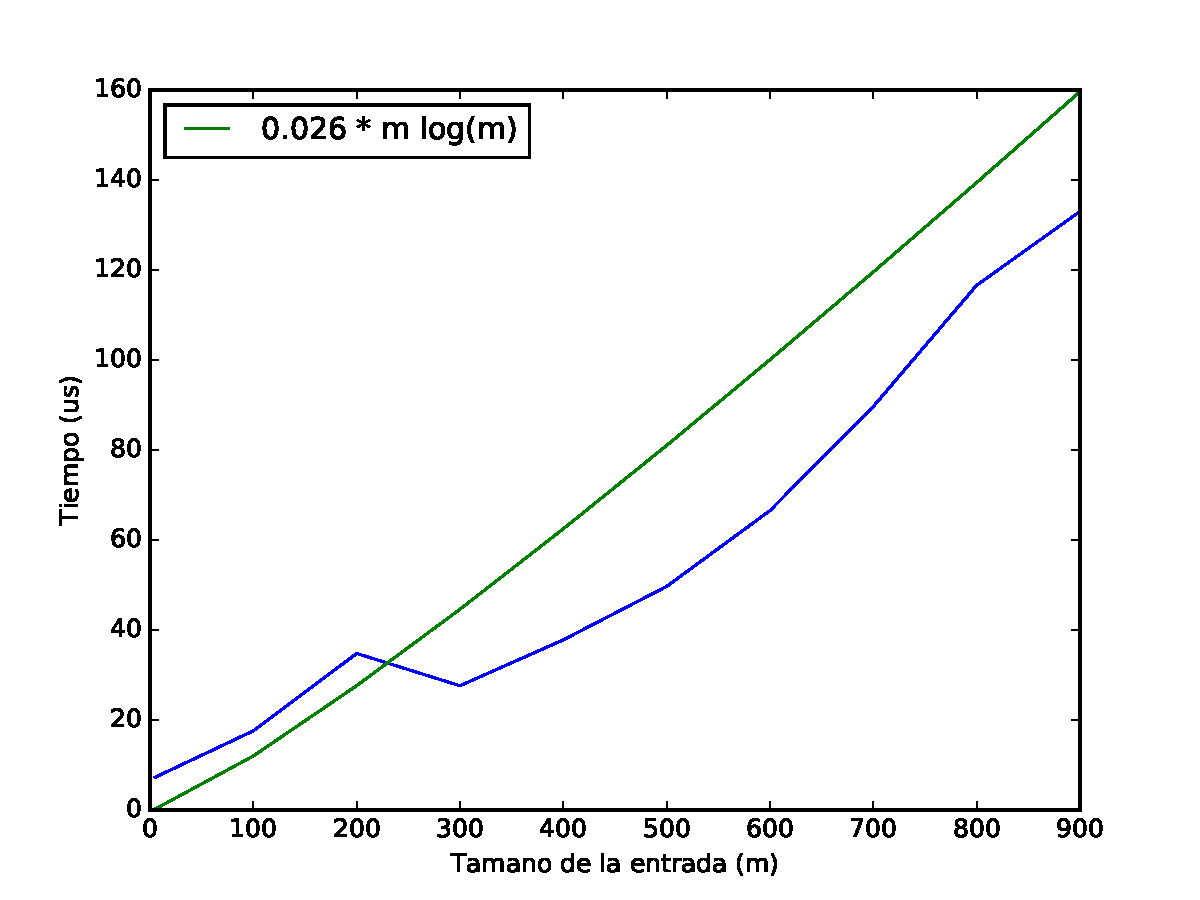
\includegraphics[width=0.9\textwidth]{img/exp/problema2-promedio.pdf}
	\caption{\footnotesize Tiempo que toma el algoritmo en $\mu$s para una entrada de tamaño $m$. $n$ al azar.}
	\label{fig:problema2-promedio}
\end{figure}

\begin{figure}[H]
 \centering
	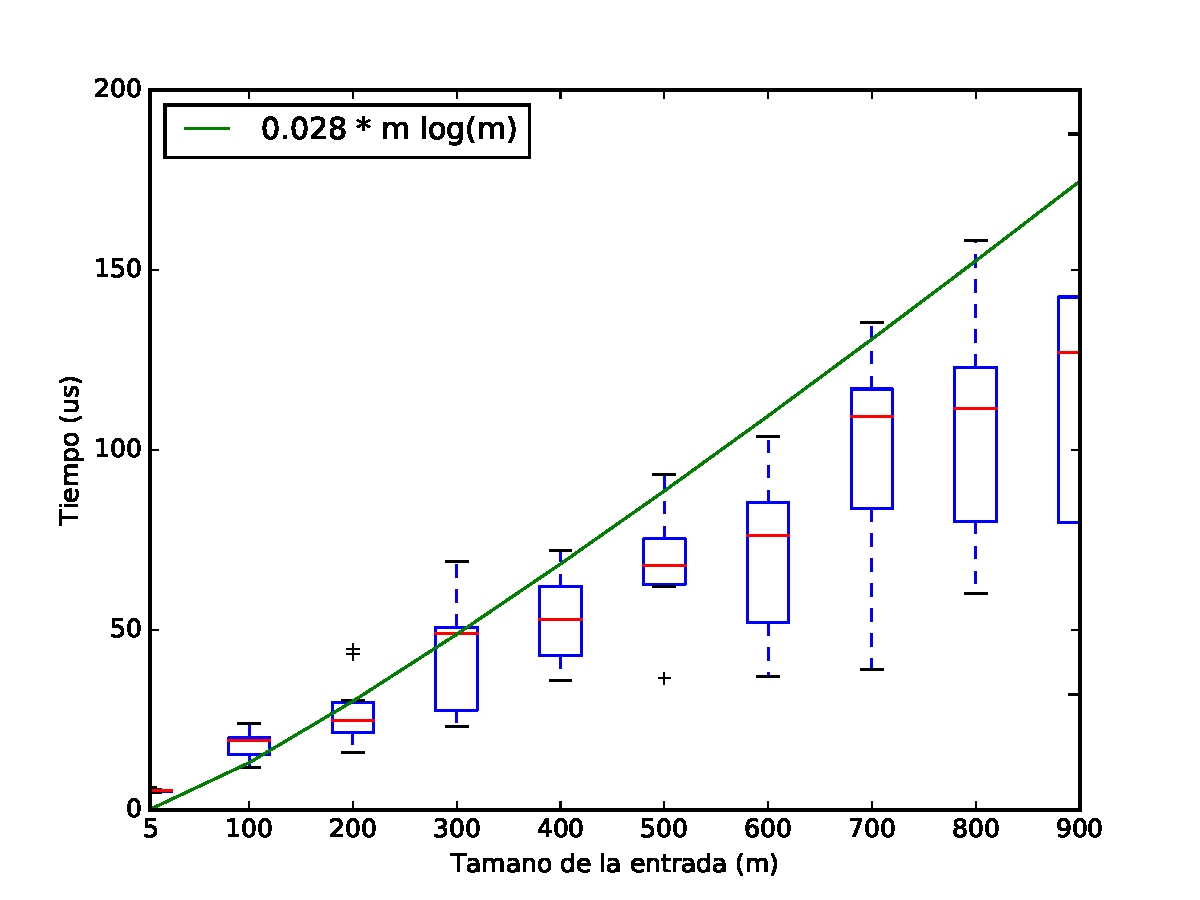
\includegraphics[width=0.9\textwidth]{img/exp/problema2-promedio2.pdf}
  \caption{\footnotesize Tiempo que toma el algoritmo en $\mu$s para una entrada de tamaño $m$. $n$ al azar. Se indican los valores del primer al tercer cuartil con un rectángulo azul y la mediana con una linea roja. El máximo y minimo se indican con lineas negras arriba y abajo del rectángulo.}
	\label{fig:problema2-promedio2}
\end{figure}

\begin{figure}[H]
 \centering
	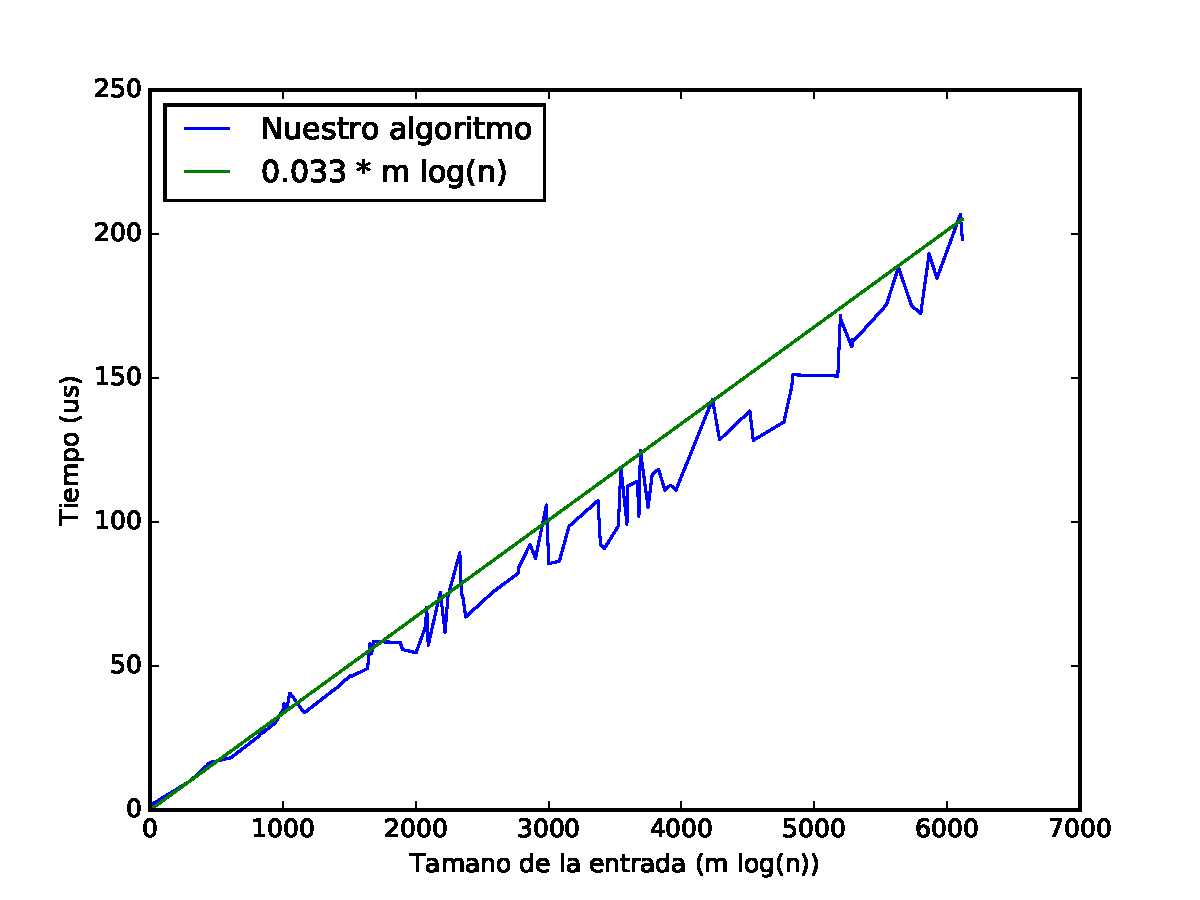
\includegraphics[width=0.9\textwidth]{img/exp/problema2-posta.pdf}
	\caption{\footnotesize Tiempo que toma el algoritmo en $\mu$s para una entrada de tamaño $m \log n$.}
	\label{fig:problema2-posta}
\end{figure}


\subsubsection{M\'etodo de experimentación}
